\section{Operatives Projektcontrolling}
\label{sec:opc}
In diesem Kapitel wird das operative Projektcontrolling orientiert an den Lebenszyklusphasen eines einzelnen Projektes beschrieben. Die Sicht auf die Planung wird um die Aspekte der Steuerung und Kontrolle ergänzt.[...]tbd
\subsection{Operative Projektplanung}
\label{ssec:opp}
\begin{quote}
\glqq Projektplanung meint die systematische Informationsgewinnung über den zukünftigen Ablauf des Projektes und die gedankliche Vorwegnahme des notwendigen Handelns im Projekt.\grqq\footnote{\cite{Platz&Schmelzer1986}, S.~132}
\end{quote}
Die Projektplanung beschränkt sich nicht auf einen einmaligen Prozess am Anfang eines Vorhabens, sondern wird projektbegleitend durchgeführt\footnote{Vgl. \cite{Fiedler2008}, S.~100}. D. h. die Planung bezieht sich einerseits auf den Projektgegenstand und andererseits auf den Projektablauf\footnote{Vgl. \cite{Litke2007}, S.~153}. Im Verlauf der Projektrealisierung dient der Projektplan als Grundlage für Fortschrittskontrollen und Projektbewertungen, die ohne einen solchen Plan unmöglich wären. Der kontinuierlich den aktuellen Gegebenheiten angepasste Projektplan konvergiert zum Projektende gegen den Ist-Zustand\footnote{Vgl. \cite{Gubbels2006}, S.~8}
\begin{table}
\begin{center}
\caption[Überblick über die operative Projektplanung]{Überblick über die operative Projektplanung}

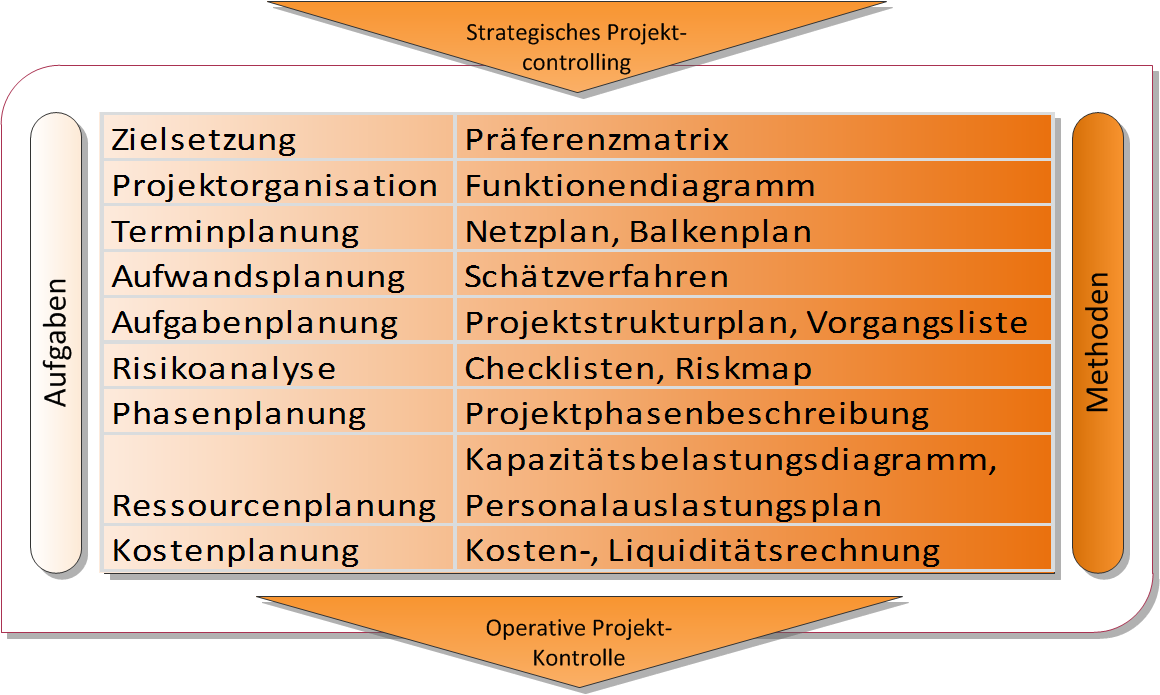
\includegraphics[width=0.8\textwidth]{Images/opPlanung.png}
\label{tbl1}

   {\footnotesize In Anlehnung an: \cite{Fiedler2008}, S. 100}
\end{center}

\end{table}

Die Tabelle \ref{tbl1} auf Seite \pageref{tbl1} zeigt einen Überblick über die verschiedenen Aufgaben und Methoden innerhalb der operativen Projektplanung. 
Der Projektleiter ist für die Planung verantwortlich\footnote{Vgl. \cite{Kuster&Huber2011}, S.~148}. Im Folgenden werden die Aufgaben des Projektcontrollings herausgestellt und abgegrenzt.

Die grundsätzlichen Regelungen für die Planungen wird durch das operative Projektcontrolling erarbeitet. Dazu gehört die verbindliche Vorgabe, dass kein Projekt ohne Projektauftrag mit Zielplanung gestartet wird.\footnote{Vgl. \cite{Fiedler2008}, S.~101}. 

%\begin{quote}
%Das Projektcontrolling kann Kriterien(z. B. Größe, Komplexität,Bedeutung des Projekts) für die Wahl der Projektorganisation erar-beiten.Im Rahmen der Planung wirdder Projektleiterunterstützt, um diefür das Projekt erforderlichen Personen zu finden. In der Matrixor-ganisation tritt manchmal das Problem auf,dass die Mitarbeiternicht in ausreichendem Maße von ihren Fachabteilungsaufgabenentlastet werden. Der Projektcontroller achtet deshalb frühzeitigdarauf,dass Vereinbarungen zwischen Projektleiterund Fachbe-reichsleitung zur Freistellung der Mitarbeiter getroffen und eindeu-tig dokumentiert werden.\footnote{\cite[S.~102]{Fiedler2008}}
%\end{quote}
%\begin{quote}
%Da die Aufgabenstruktur vieler Projekte vergleichbar ist, sollte dasProjektcontrollingeinen Standardprojektstrukturplan erarbeiten.Die Anpassung an einneues Projekt ist schnell durchführbar, indemeinfach die nicht benötigten Arbeitspaketeentferntund neue dazu-gefügt werden. So erhält man schnell einen aktuellen Planmit Aus-gangsdaten für die Termin- und Kostenplanung.Die folgende Abb. 83 zeigt im Überblick die Gliederung der Ebenendes Standardstrukturplans für das Projektgeschäft der FAG Kugelfi-scher AG  Co. KG. 
%Das Projektcontrolling kann auch formale Standards für die Defi-nition von Projektstrukturplänen vorgeben:• Eine Aktivität muss immer aus einem Hauptwort und einemVerbbestehen, z. B. "Bremsenprüfen".• Ein Meilenstein ist als Ereignis zu formulieren, z. B. "Bremsengeprüft".• Dieerste Ebene ist mit Großbuchstaben zuschreiben, um dieÜbersichtlichkeit zu erhöhen.• Auf der ersten Ebene dürfen keine Arbeitspaketeerscheinen.• Dieerste Ebene umfasst immer diegleichen, zentral vorgegebe-nen Standardvorgänge.• Essind höchstenssechs Gliederungsebenen zulässig. 
%Das Projektcontrolling hat im Rahmen der Koordination die korrek-te Definition der Meilensteine dahingehend zu prüfen, ob sie mitdem Projektauftrag korrespondierenoder vertraglich zugesicherteLeistungstermine berücksichtigen. Außerdemmuss die Vollstän-digkeit des Projektstrukturplans begutachtet werden. Technischorientierte Projektleiter übersehen schnell vertriebliche und organi-satorische Aufgaben.Der Projektcontrollerunterstützt darüber hinaus die Abstimmungder Rahmen- und Detailpläne.\footnote{\cite{Fiedler2008}}
%\end{quote}\begin{quote}
%Als gestaltende Maßnahme muss das Projektcontrollingeine Ter-minplanung mit ausreichendem Detaillierungsgrad für jedesProjekt verbindlich fordern. Ergänzend sollten Empfehlungen fürden Einsatzvon Balkenplänen und Netzplandiagrammen formuliertwerden. Hinweise auf geeignete DV-Instrumente gewährleistenine effiziente und einheitliche Terminplanung.Der Projektcontroller kann auch die Machbarkeit des Terminplansprüfen. Insbesondere sollteer darauf achten, ob genügend Ressour-en zu den geplanten Zeitpunkten bereitstehen. Es ist auch sicher zutellen,dass die Ressourcenprojektübergreifend entsprechendderProjektprioritätenoptimal eingesetzt werden.Ein besonderes Augenmerk sollte der Projektcontroller auf dieein-geplanten Pufferrichten.\footnote{\cite[S.~130]{Fiedler2008}}
%\end{quote}\begin{quote}
%Das Projektcontrolling sollte die realistische Ermittlung und zen-trale Dokumentation der freien Kapazitäten sicherstellen. Damitwird auch eine ungleichmäßige Ressourcenauslastung vermieden. Inder Praxis kommt es immer wieder vor,dass einige Mitarbeiter zumehr als 100 Prozent ausgelastetsind, während andere noch freieKapazitäten haben.Diefür ein Projekt zur Verfügung stehende Zeit eines Mitarbeiterswird manchmal zu optimistisch gesehen. Gründe sind:• Es wirddiegesamte Bruttoarbeitszeit eingeplant.• Offiziell abgeschlossene Projekte binden weiterhin Kapazitätendes Mitarbeiters.• Urlaub und Krankheitstage werden übersehen. 
%Das Projektcontrolling sollte dazu beitragen,diese Probleme auf-zudecken.Erkennt der Projektcontroller Engpässe, muss er dafürsorgen,dassdiesefrühzeitig kommuniziert undbeseitigt werden.Es ist vor allem beiknappen Ressourcen erforderlich,dass eine pro-jektübergreifende Koordination des Mitarbeitereinsatzes erfolgt.Wertvoll ist es in dieser Situation, wenn die Prioritäten der Projektebekanntsind (vgl. Abschnitt 2.1).Der Projektcontrollersollte auch dafür Sorge tragen,dass dieein-zelnen Mitarbeiter nicht in zu vielen Projekten eingesetzt werden.Verplant man den Mitarbeiter inmehr als fünf Projekten, sindderKoordinierungsaufwand unddie durch den Wechsel zwischen denverschiedenen Aufgaben bedingten "geistigen Rüstzeiten" zu hoch.Wenn ein Mitarbeiter mit weniger als20 Prozent zur Verfügungsteht, ist auch das Interessefür das Projekt gering.In einer Projektmatrixorganisation,bei der ein Mitarbeiter nebendem Projekt auch noch sein Tagesgeschäft erledigenmuss, ist vonvornherein sicherzustellen,dass er in seiner Fachabteilung auchimerforderlichen Umfangentlastet wird. Geschieht das nicht, wirdderMitarbeiterschnell überfordert, mit der Folge,dass seine Motivationim Projektsinkt. Um diese Situation zu vermeiden, kann der Pro-jektcontroller einen Kontrakt zwischen ProjektleiterunddenAbteilungsleitern anregen, in dem diese sich verpflichten,die Mit-arbeiter entsprechend ihrer Projekteinplanung vom Tagesgeschäftfreizustellen.\footnote{\cite[S.~152--153]{Fiedler2008}}
%\end{quote}


\subsection{Operative Projektkontrolle}
Projektkontrolle hat die Aufgabe der Schaffung von Transparenz mittels eines effizienten Reportings und die Entscheidungsvor-- und --nachbereitung.\\Voraussetzung sind eine realistische, vollständige und nachvollziehbare Projektplanung (Vgl. Kapitel \ref{ssec:opp}). Den quantifizierbaren Größen der Projektkontrolle sind die Bewertungsdimensionen des magischen Dreieck (Vgl. Abb. \ref{abb2}, S. \pageref{abb2}) zu Grunde gelegt\footnote{Vgl. \cite{Bergmann&Garrecht2008}, S.~228}. Um mögliche Abweichungen vom geplanten Projektablauf zu erkennen, werden die Ist-Werte den ursprünglich geplanten Werten gegenübergestellt. Kommt es zu Abweichungen vom Plan, so erfolgt eine erneute Projektplanung auf Grundlage der aktualisierten Daten. Besteht die Gefahr, dass wichtige Abschlusstermine nicht eingehalten oder dass bestimmte Kostenziele überschritten werden, muss das Projektmanagement Maßnahmen entwickeln, um auf solche Abweichungen geeignet reagieren zu können\footnote{Vgl. \cite{Zimmermann&Rieck&Stark2006}, S.~107}
\begin{table}
\begin{center}
\caption[Elemente der Projektkontrolle]{Elemente der Projektkontrolle}

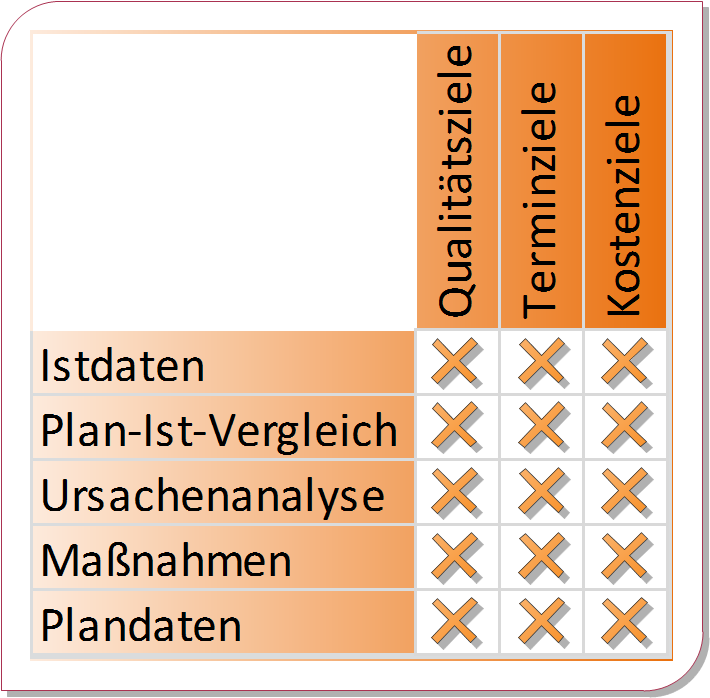
\includegraphics[width=0.4\textwidth]{Images/elementeSteuerung.png}
\label{tbl2}

   {\footnotesize In Anlehnung an: \cite{Fiedler2008}, S. 177}
\end{center}

\end{table}
Die Abbildung \ref{abb8} auf Seite \pageref{abb8} zeigt das Zusammenspiel der operativen Projektplanung und -kontrolle als Fundierung der Projektsteuerung. 
Die Projektkontrolle beinhaltet folgende Aufgaben(vgl. Abb. \ref{abb8})\footnote{Vgl. \cite{Fiedler2008}, S. 176}:
\begin{compactitem}
\item Ermittlung der Istdaten,
\item Gegenüberstellung der entsprechenden Plandaten,
\item Untersuchung der aufgetretenen Abweichungenmit dem Ziel, deren Ursachen herauszufinden, und gegebenenfalls
\item Planung und Einleitung von Gegenmaßnahmen.
\end{compactitem}
\begin{figure}[htbp]
%\begin{floatingfigure}[r]{0.7\textwidth}
\begin{center}
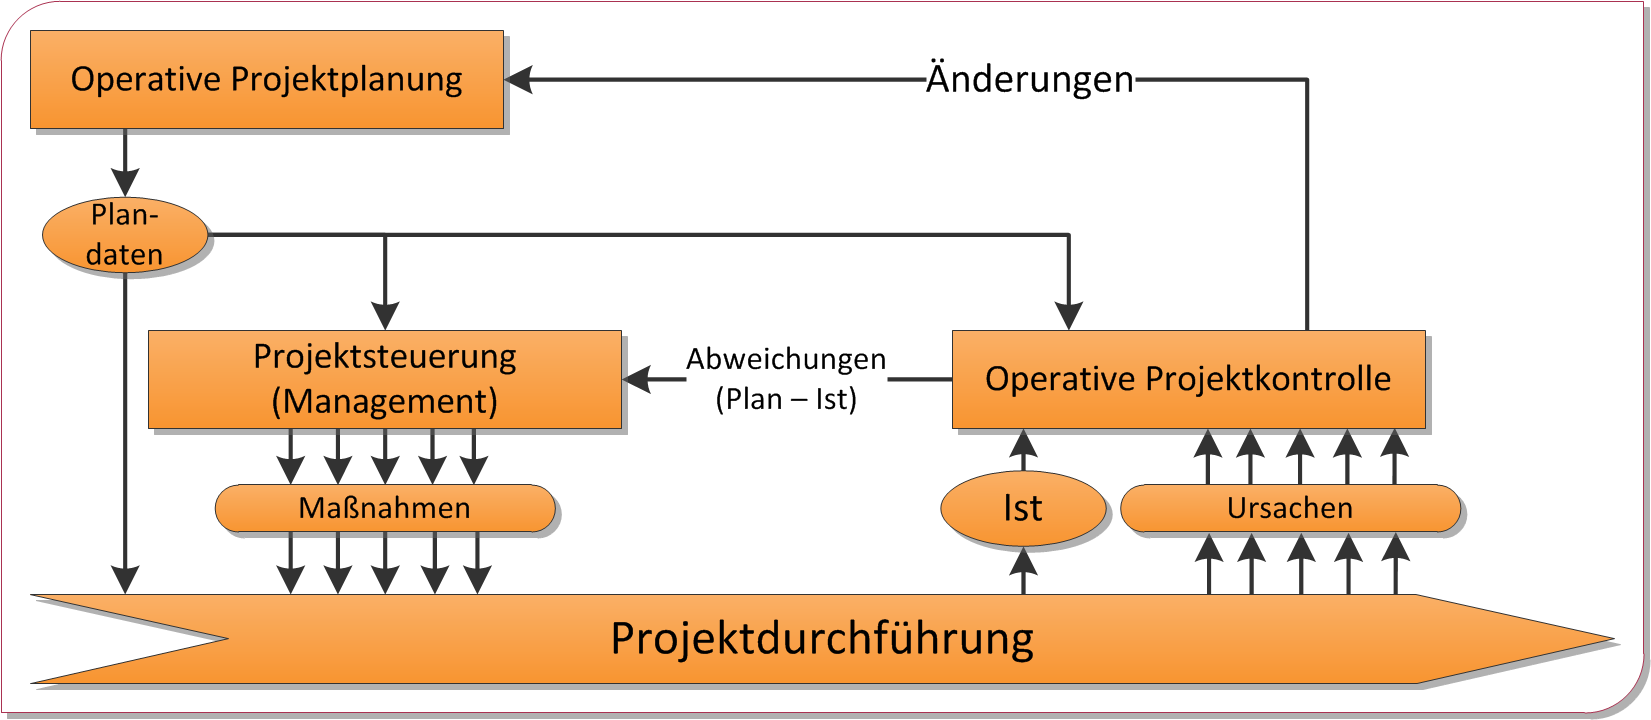
\includegraphics[width=1\textwidth]{Images/Steuerung.png}
{\footnotesize In Anlehnung an: \cite{Litke2007}, S. 84}
\caption[Modell der Projektlenkung]{Modell der Projektlenkung}\label{abb8}
\end{center}
\end{figure}
%\end{floatingfigure}
Nach Frank Lüschow und Elke Zitzke ist der Projektleiter auf die realistische Einschätzung seiner Teammitglieder angewiesen, um den Ist-Zustand im Projekt realistisch einschätzen zu können. An dieser Stelle ist der Projektleiter auf seine eigene und die Intuition seiner Teammitglieder angewiesen. Um an diese Informationen heranzukommen, muss er laufend aktiv Kontakt zu seinen Teammitgliedern halten. Diese Methode wird von den Autoren zusammengefasst als:\begin{quote}\glqq Controlling by walking around\grqq\footnote{\cite{Luschow&Zitzke2004}, S.~102}\end{quote}
Diese Methode ist nach Lüschow und Zitzke ein Teil der Kontrolle und wird durch messbare Daten gestützt\footnote{Vgl. \cite{Luschow&Zitzke2004}, S.~101--102}. Rudolf Fiedler bewertet die intuitive Einschätzung des Projektleiters und der Mitarbeiter weitaus kritischer. Er nimmt Bezug auf das 90\%- oder Fast-schon-fertig Syndrom und gibt zu Bedenken, dass der erreichte Fertigstellungsgrad oft zu hoch eingeschätzt wird, obwohl eine nicht mehr auszugleichende Planabweichung vorliegt\footnote{Vgl. \cite{Litke2007}, S.~181--182)}. \abk{90\%-Syndrom}{häufige Fehleinschätzung des Fertigstellungsgrades}
Unumstritten ist, dass für effizientes Projektcontrolling nicht nur ex-post 
durch Kontrolle und Überwachung Abweichungen festzustellen, sondern das 
Auftreten von Abweichungen antizipativ erst gar nicht entstehen zu lassen. Für diesen proaktiven Ansatz der Projektsteuerung empfiehlt es sich die Trends des Fortschritts in Besprechungen mit dem Projektteam regelmäßig abzufragen\footnote{Vgl. \cite{Bergmann&Garrecht2008}, S.~229}. 
\subsubsection{Einhaltung des Terminziels}
Eine Form der Darstellung des Plan-Ist-Vergleichs der Terminerreichung ist die Meilenstein-Trendanalyse (Abbildung \ref{abb9}, Seite \pageref{abb9}). In dieser Form der Darstellung wird die Erreichung der Meilensteine aufgeführt. An den Achsen werden die im Projektplan festgelegten Meilensteine (Ordinate) und die Berichtstermine (Abszisse) in zeitlich aufsteigender Folge eingetragen. Bei Erreichen der jeweiligen Berichtstermine wird die Abbildung weiter vervollständigt. Wenn im Laufe des Projektes die Planeinhaltung nicht mehr realistisch erscheint und es eine aktualisierte Erwartung gibt, so wird auf den neuen Erkenntnissen ein aktualisierter Plan aufgesetzt. Dieser Ausblick wird Forecast \abk{Forecast}{Ausblick/Prognose auf erwartete Ergebnisse nach aktuellen Erkenntnissen} genannt, in den Spalten zu den jeweiligen Berichtsterminen eingetragen und mit einer Linie verbunden\footnote{Vgl. \cite{Wegmann&Winklbauer2006}, S.~191--192}. Auf Basis des Kurvenverlaufs ist eine Termineinschätzung möglich\footnote{Vgl. \cite{Litke2007}, S.~156}:
\begin{compactitem}
\item Fallender Verlauf: Termin wird unterschritten.
\item Waagerechter Verlauf: Termin wird eingehalten.
\item Ansteigender Verlauf: Termin wird überschritten.
\end{compactitem}

\begin{figure}[htbp]
%\begin{floatingfigure}[r]{0.7\textwidth}
\begin{center}
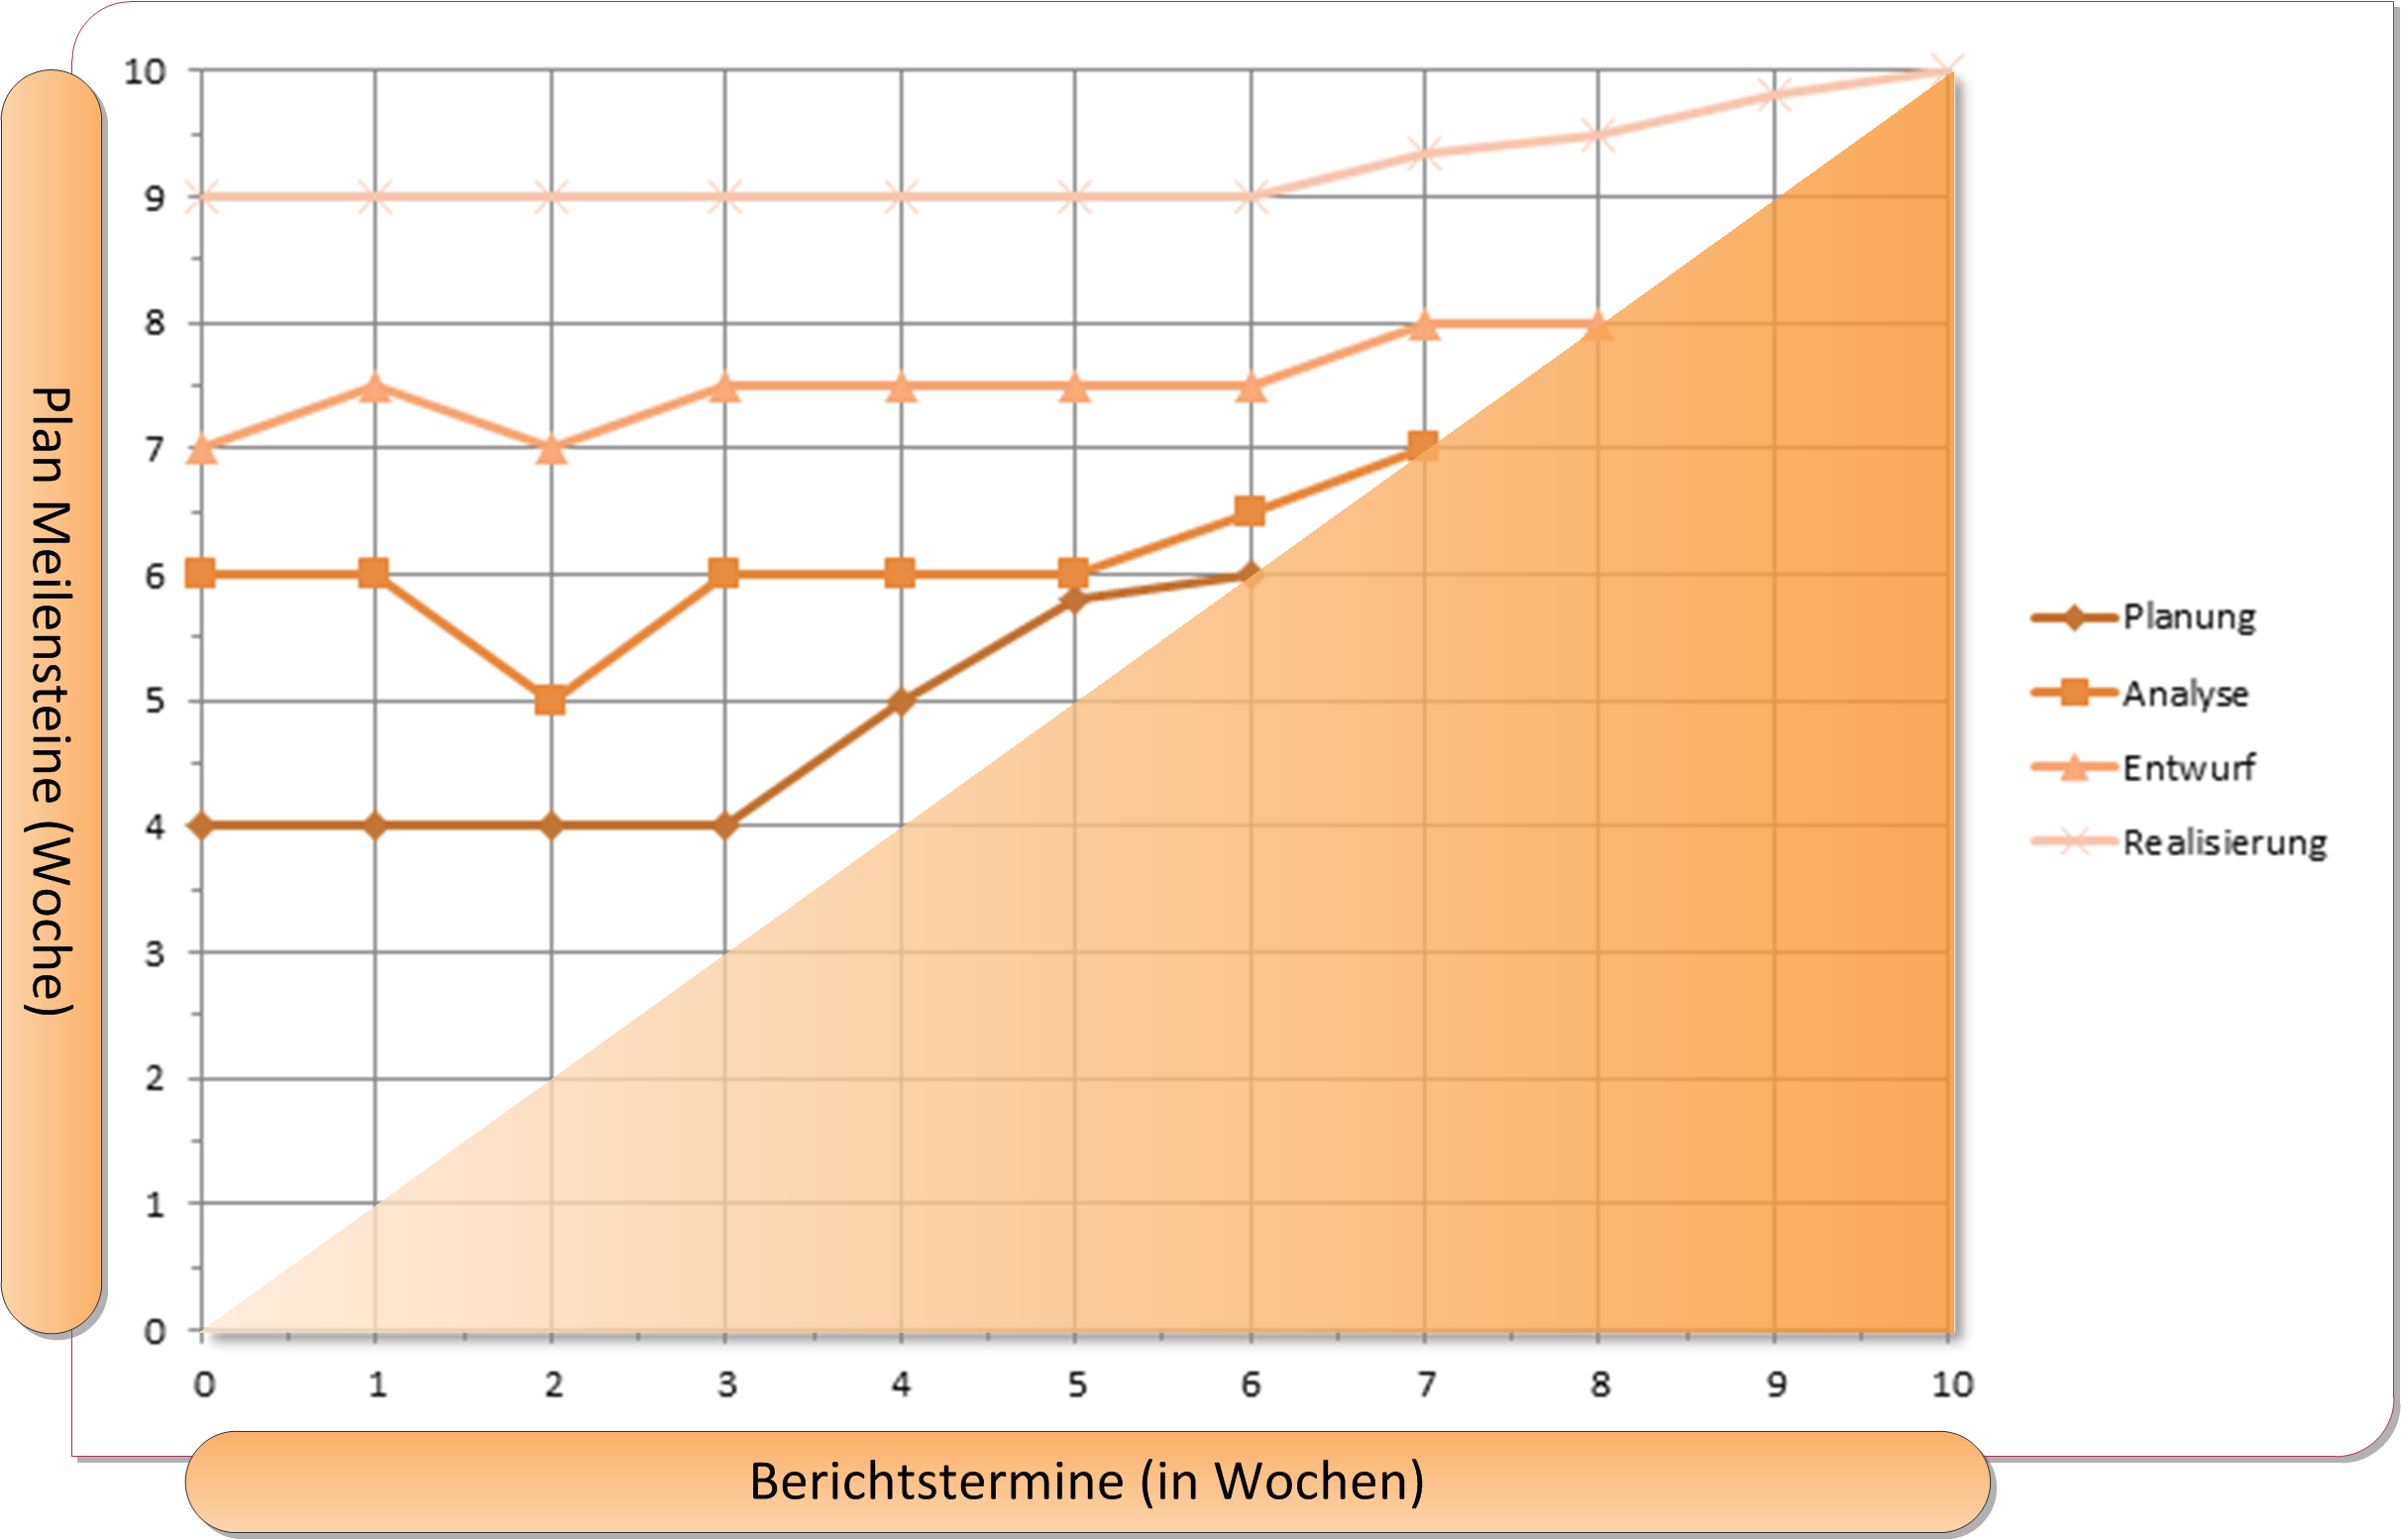
\includegraphics[width=0.8\textwidth]{Images/trendAnalyse.png}\\{\footnotesize In Anlehnung an: \cite{Blazek2001}, S. 152}
\caption[Meilenstein-Trendanalyse]{Meilenstein-Trendanalyse}\label{abb9}
\end{center}
\end{figure}
%\end{floatingfigure}

\subsubsection{Einhaltung des Qualitätsziels}
Für die Erfassung des Qualitätsziels stehen eine Reihe von Methoden und Techniken zur Verfügung. Eine besonders einfache Methode ist die Meilensteinmethode. Man zählt die bisher erreichten Meilensteine und setzt sie mit der Gesamtzahl der Meilensteine in Bezug. Sie die Meilensteine genügend differenziert, kann diese Form der Erfassung zufrieden stellende Ergebnisse liefern. Die Planabweichung wird dabei durch die zeitliche Bindung der Meilensteine deutlich und kann durch die Division der Ist- durch die Planwerte als Kennzahl des Fortschrittsgrades dargestellt werden\footnote{Vgl. \cite{Fiedler2008}, S.~182}.

Genauere Ergebnisse können mit dem Fokus auf die geplanten Arbeitspakete erzielt werden. Es wird die Planmäßigkeit der abgeschlossenen Arbeitspakete bewertet (0/100-Methode). Alternativ kann auch der Fortschritt innerhalb eines Arbeitspaketes bewertet werden. Man wählt hier Vorgehensweisen wie die 0/50/100-Methode, um dem 90\%-Syndrom angemessen zu begegnen\footnote{Vgl. \cite{Fiedler2008}, S.~183}.
Ein Beispiel zur Darstellung des aktuellen Projektfortschritts in MS-Project ist im Anhang 2 (Kapitel \ref{sec:Anhang2}, Seite \pageref{sec:Anhang2}) zu finden.

Oft wird die bereits erbrachte Leistung zu positiv eingeschätzt. Es bietet sich an, die noch zu erbringende Leistung als zukunftsorientierter Indikator der Qualität zu wählen\footnote{Vgl. \cite{Luschow&Zitzke2004}, S.~102}. Die Effort-Expended-Methode gibt den Leistungsmäßigen Fortschrittsgrad (FG) nach folgender Formel aus\footnote{Vgl. \cite{Fiedler2008}, S.~183}: $FG = \frac{Istaufwand*100}{Vorraussichtlicher Gesamtaufwand}$

\subsubsection{Einhaltung des Kostenziels}
Die Kostenkontrolle legt den Fokus auf die zum aktuellen Zeitpunkt erwarteten Kosten und vergleicht sie mit den tatsächlich angefallenen Kosten. Die Voraussetzung für aussagekräftige Auswertungen sind eine hohen Planungs- und Erfassungsqualität der Kosten. Eine einfache Variante eines Plan-Ist-Vergleich ist im Anhang 1 (Kapitel \ref{sec:Anhang1}, Seite \pageref{sec:Anhang1}) zu finden. Die Abbildung \ref{abb10} auf der Seite \pageref{abb10} zeigt eine zusammengefasste Sicht mit Forecast aus der Perspektive des gesamten Projektes\footnote{Vgl. \cite{Wegmann&Winklbauer2006}, S.~182--183}.
\begin{figure}[htbp]
%\begin{floatingfigure}[r]{0.7\textwidth}
\begin{center}
\includegraphics[width=0.8\textwidth]{Images/Forecast.png}\\{\footnotesize In Anlehnung an: \cite{Blazek2001}, S. 142}
\caption[Kostentrendanalyse]{Kostentrendanalyse}\label{abb10}
\end{center}
\end{figure}
%\end{floatingfigure}


\subsubsection{Earned Value Analyse}
\begin{table}[htbp]
%\begin{floatingfigure}[r]{0.7\textwidth}
\begin{center}
\caption[Abkürzungen Earned Value Analyse]{Abkürzungen Earned Value Analyse}\label{tbl3}
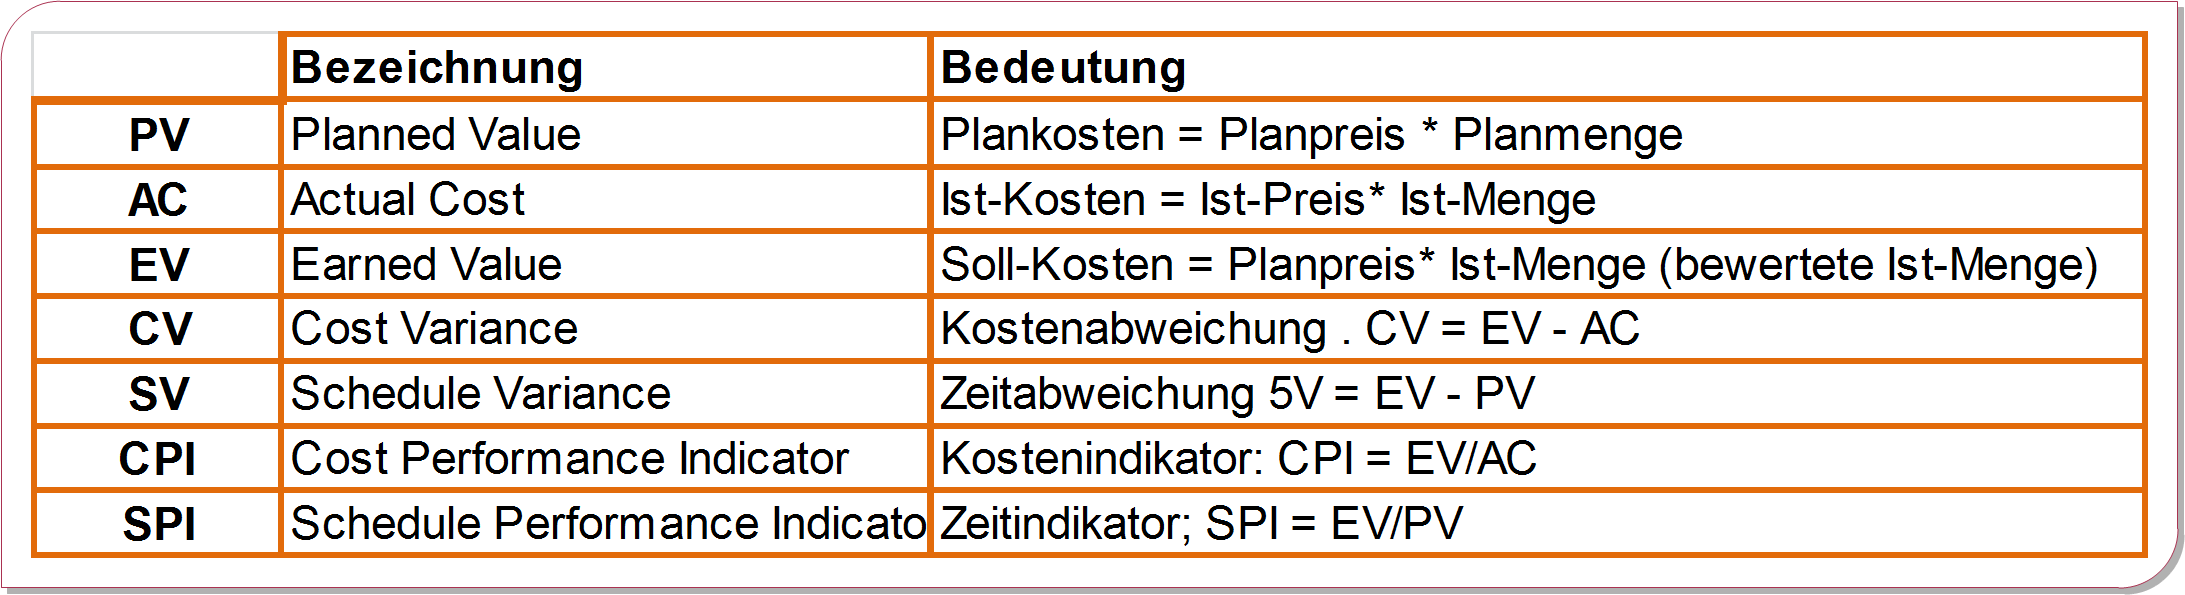
\includegraphics[width=0.8\textwidth]{Images/ev.png}\\{\footnotesize In Anlehnung an: \cite{Drews&Hillebrand2007}, S.~233}
\end{center}
\end{table}
In den vorangegangenen Kapiteln wurden Methoden aufgezeigt, die die Dimensionen des magischen Dreiecks einzeln überwachen. Am Beispiel der Kostenanalyse in Abbildung \ref{abb9} auf Seite \pageref{abb9} kann man nicht erkennen, ob die höheren Kosten zum Zeitpunkt der Erfassung auf einen schnellere oder eine unwirtschaftliche Leistungserbringung (Qualitätsziel) zurückzuführen ist. 
Das Beispiel verdeutlicht, dass die Kostenkontrolle auch die Erfüllung des Qualitätsziel mit einbeziehen muss. Dies erreicht man durch den Ausweis von Sollkosten für jedes Arbeitspaket. Das sind diejenigen Kosten, die für eine gegebene Leistung zum planmäßigen Termin anfallen dürfen. Man spricht auch vom so genannten Earned Value\footnote{Vgl. \cite{Fiedler2008}, S.~198}.
Die Earned-Value-Analyse berücksichtigt alle drei Dimensionen des magischen Dreiecks. Sie bedient sich dazu folgenden Kategorien: den Ist-Kosten, den Plankosten und den Soll-Kosten (Earned Value). Mit diesen drei Kategorien ermittelt die Earned-Value-Analyse die Kostenabweichung (Cost Variance) im Projekt. Die Kennzahl der Zeitabweichung wird als Schedule Variance bezeichnet. Die Kostenabweichung errechnet sich aus der Differenz der Soll-Kosten zu Ist-Kosten und zeigt die Abweichung der tatsächlichen Kosten zu den geplanten Kosten der erreichten Qualität. Die Zeitabweichung ermittelt sich aus der Differenz von Soll-Kosten - Plankosten\footnote{Vgl. \cite{Drews&Hillebrand2007}, S.~232}.
%\end{floatingfigure}
\begin{figure}[htbp]
%\begin{floatingfigure}[r]{0.7\textwidth}
\begin{center}
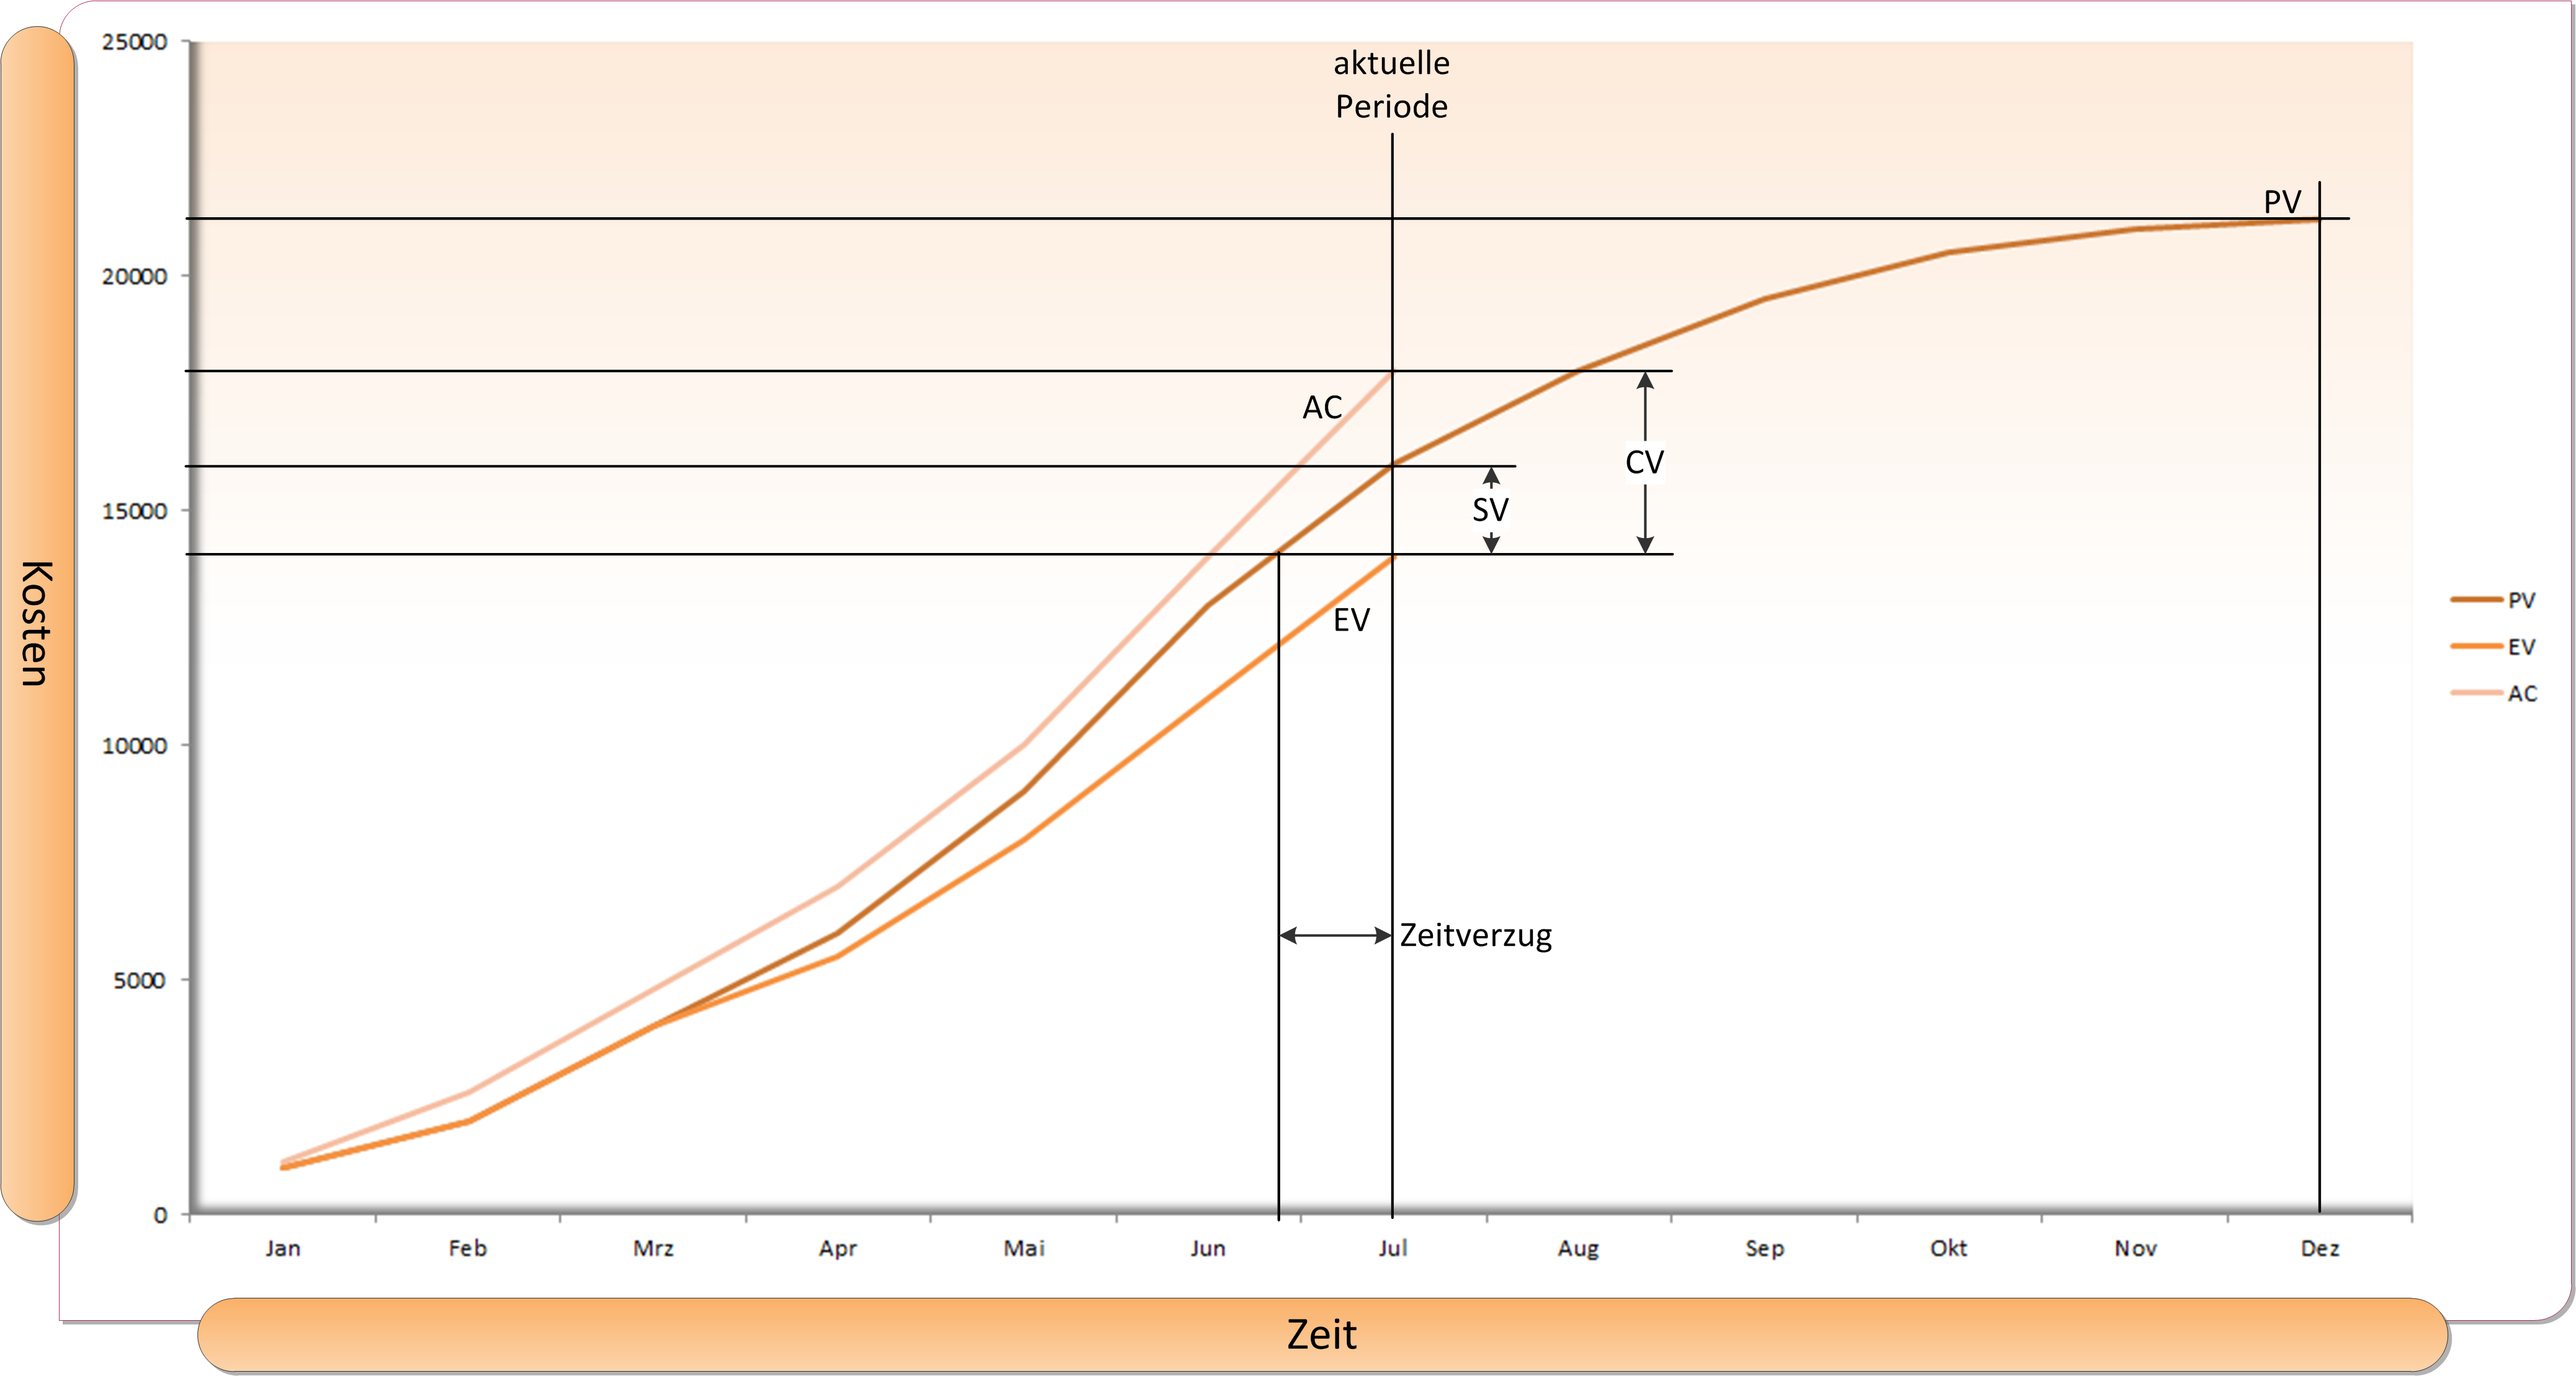
\includegraphics[width=1\textwidth]{Images/eva.png}\\{\footnotesize In Anlehnung an: \cite{Drews&Hillebrand2007}, S. 234}
\caption[Earned Value Analyse]{Earned Value Analyse}\label{abb11}
\end{center}
\end{figure}
%\end{floatingfigure}

Die Abbildung \ref{abb11} auf Seite \pageref{abb11} zeigt die Anwendung des Kennzahlensystems aus Tabelle \ref{tbl3} auf Seite \pageref{tbl3}. Mit den Größen der Earned Value Analyse lassen sich wie in der Meilensteintrendanalyse Aussagen zur Terminerreichung und wie in der Kostentrendanalyse Aussagen zum Kostenverlauf machen. Alle drei Werkzeuge bilden gemeinsam ein wichtiges Instrumentarium, um absolute Zahlen und Trends ermitteln zu können\footnote{Vgl. \cite{Gubbels2006}, S.~34}. 